\documentclass[12pt]{article}

\usepackage{fullpage}
\usepackage{graphicx, rotating, booktabs} 
\usepackage{times} 
\usepackage{natbib} 
\usepackage{indentfirst} 
\usepackage{setspace}
\usepackage{grffile} 
\usepackage{hyperref}
\usepackage{adjustbox}
\usepackage{amsmath}
\setcitestyle{aysep{}}


\singlespace
\title{\textbf{Alliance Participation and Military Spending}}
\author{Joshua Alley\footnote{Graduate Student,
Department of Political Science, Texas A\&M University.}}
\date{{\normalsize \today}}

\bibliographystyle{apsr}

\begin{document}

\maketitle 

\newpage 

\doublespace 

\begin{abstract}
How does alliance participation impact military spending? 
Previous scholarship on this question is divided between competing assertions that alliance participation increases or decreases military spending. 
I argue that alliance participation can raise or lower military expenditures in different circumstances. 
Increasing treaty strength leads major powers to reduce growth in military spending because they use alliances for international influence. 
Non-major powers increase growth in military spending because they use alliances to secure their territory. 
I test this argument by creating a measure of alliance treaty strength and employing that measure in a multilevel model. 
The multilevel model generates novel empirical evidence linking alliance participation and growth in state military spending from 1816 to 2007. 
I find that greater treaty strength increases growth in military spending in non-major powers and decreases spending growth in major powers.  
\end{abstract}



\section{Introduction}


How does alliance participation affect military spending? 
Scholarship on this issue is divided between two camps. 
The force multiplier perspective expects alliance participation to reduce military spending. 
The foreign entanglement group predicts alliances participants will spend more on defense. 


In this paper, I address the division between these two perspectives on alliance participation and military expenditures. 
I show when alliance participation increases and decreases growth in military expenditures, thereby making a theoretical and empirical contribution. 
I argue that major and non-major power states use alliances for different purposes, so they respond differently to changes in treaty strength.


Major powers use strong treaty commitments to increase their influence. 
Strong treaties replace military spending as a source of influence, allowing large states to reduce spending. 
Non-major powers emphasize territorial security from alliances.  
These small states sacrifice the freedom to reduce military spending for greater security from a strong treaty. 
Weaker treaties still provide less security without tying military support to other costly commitments, giving non-major powers the chance to reduce military spending. 


I test these predictions with a novel research design.
The first empirical contribution is a latent measure of alliance treaty strength. 
I then incorporate that measure into a multilevel model which directly compares alliance treaties, and estimates the impact of each treaty on members' military spending.
Multilevel modeling links the alliance and state levels of analysis.   


% why you should care
Unifying scholarship on alliance participation and military spending has academic and practical value.
Force entanglement and force multiplier arguments treat alliances as homogeneous, and dispute the the characteristics of alliances.\footnote{See \citet{DigiuseppePoast2016} for an important exception.} 
But there is substantial variation in alliance membership and treaty content \citep{Leedsetal2002}. 
Therefore, mutually exclusive claims alliance participation increases or decreases military spending may be misleading. 


Arguments between the foreign entanglement and force multiplier camps are a poor guide for policy discussions. 
Policy debates emphasize reduced spending by alliance members- especially US allies. 
But these debates fail to understand that reduced defense spending by US allies is the result of different incentives for large and small states. 
Maintaining US influence requires additional military spending, given the proclivity of the US and other democracies to make weaker formal commitments. 
Weak alliance commitments give security without restricting the freedom of junior partners to reduce military spending. 


The conditional argument and evidence in this paper have important implications. 
Alliance treaty design has distributional consequences because commitment strength shapes how large and small alliance members allocate resources to the military. 
Large and small members will bear different security burdens under different treaties.


Growth in military spending has domestic opportunity costs--- funds spent on security cannot be spent on other goods. 
Greater military spending impacts economic growth \citep{ShinWard1999, AlptekinLevine2012} and domestic politics \citep{Narizny2003, WhittenWilliams2011, Williams2015}.
So military spending decisions have distributional consequences in international and domestic politics. 


Another implication of this argument is that major and minor powers face different tradeoffs in alliance politics, 
Strong commitments give major powers more influence, at the risk of entrapment \citep{Benson2012}.
For non-major powers, strong treaties provide more security at the cost of freedom to reduce military spending. 


The paper proceeds as follows. 
First, I summarize the competing arguments and mixed empirical evidence on alliance participation and military spending. 
Then I describe the argument in more detail. 
The third and fourth sections describe the research design and results. 
The final section concludes with a discussion of the implications for scholarship and policy.  


\section{Force Multiplier or Foreign Entanglement?}

% 2-3 paragraphs per subsection

Scholarship on alliance participation and military spending is divided between two perspectives. 
The foreign entanglement predicts alliance participation will increase military expenditures.
The force multiplier school expects alliance participation to reduce military spending. 


\subsection{Force Multiplier} 


Force multiplier arguments start with the premise alliances and military spending both provide security.
States substitute between these two foreign policy instruments \citep{MostStarr1989}.  
Alliances provide security that states could not achieve without additional military spending \citep{Morrow1993, Conybeare1994}. 
Because military spending has opportunity costs, states rely on their allies for security and and reallocate military spending to other goods. 


Allied military capability replaces defense expenditures of member states. 
\citet{DigiuseppePoast2016} refine this logic by arguing that states will only reduce spending if their alliance is credible. 
Unreliable alliance capability cannot replace reliable domestic military spending. 


% quick para on public goods model
Another argument in the force multiplier perspective links reduced military spending to a collective action problem. 
\citet{OlsonZeckhauser1966} argue that security from an alliance is a public good, so treaty members provide suboptimal contributions of military spending. 
Each member free-rides on other states, and smaller members exploit the larger. 
Spending less allows alliance members to consume more non-defense goods, but the alliance provides less security. 


Both the substitution and public goods models expect alliance participation will reduce spending. 
These arguments are rooted in the opportunity costs of military spending. 
But the foreign entanglement group predicts alliance participation increases military expenditures, because alliances provide more than security. 


\subsection{Foreign Entanglement}


The foreign entanglement perspective is less cohesive.
These arguments generally focus on non-security benefits of alliance participation. 
States then use additional military expenditures to reinforce gains from alliance participation. 


% Crap ton of models- one sentance for each. add more detail later if needed. 
\citet{Diehl1994} argues that alliances increase a states foreign policy responsibilities, necessitating extra military spending. 
Because alliances expand what a state can achieve in international relations, states will increase military spending to pursue other foreign policy goals \citep{MorganPalmer2006}. 
\citet{Horowitzetal2017} show that some states increase defense effort to make themselves a more attractive alliance partner, which is a more security-focused argument. 
Others assert that alliances generate cooperation, leading to higher defense spending \citep{Palmer1990, QuirozFlores2011}
Last, \citet{SeneseVasquez2008} argue that military spending and alliances are part of a conflict spiral that produces simultaneous growth in military expenditures and alliance participation. 


Arguing alliances do more than provide security provides a crucial insight.
However, the foreign entanglement perspective does not consider the opportunity costs of military spending. 
If military spending has opportunity costs, states have incentives to reduce spending where possible.  
Likewise, the force multiplier perspective does not acknowledge synergies between military spending and alliances. 


\subsection{Mixed Evidence} 


Arguments about alliance characteristics could be settled by a preponderance of empirical evidence. 
Unfortunately, the divided state of theory is reinforced by mixed empirical results.\footnote{Because tests of the public goods model regress military spending as a share of GDP on GDP, I ignore most tests of the public goods theory of alliances in summarizing prior results. These studies are subject to an identification problem.}
Some studies find a positive association between alliance participation and military spending. 
Others find a negative relationship. 


% Specific and general studies
The wide range of methodologies and samples in previous studies can be divided into into specific and general research designs.  
Specific studies examine the impact of a few alliances, usually by tracking how a state responds to the military spending of a key ally. 
General studies compare many states using dummy indicators of alliance participation. 
Each design has different virtues and shortcomings. 


% Virtues and shortcomings- Specific studies of substitution theory of FP
A specific study examines how states respond to changes in allied capability in a few alliances. 
Most support for the substitution of arms and alliances comes from specific designs \citep{BarnettLevy1991, Morrow1993, Sorokin1994, PluemperNeumayer2015}. 
But other specific studies find increased spending by alliance members \citep{ConybeareSandler1990, Chenetal1996}. 
Specific designs provide detailed evidence, but lack generalizability. 


% General models- again, mixed results
General models capture a wide range of state-year observations and compare states with an alliance to those without.
Dummy indicators of alliance participation in a general study lump diverse treaties together in a state-level measure. 
Therefore, general studies cannot distinguish between alliances or make inferences about particular treaties. 


\autoref{tab:results-sum} summarizes previous results from general models of alliance participation and military spending. 
Like specific studies, general studies produce mixed results. 
Work by \citet{DigiuseppePoast2016} and \citet{Horowitzetal2017} provides the most reliable estimates. 


\begin{table}[hbt!]
\begin{center}
\begin{tabular}{lccc}
     & Decrease & Increase & Null \\
\hline
\citet{MostSiverson1987} &  &  & X \\
\citet{Conybeare1994} & X & &  \\
\citet{Diehl1994} &  & X &  \\
\citet{Goldsmith2003} &  &  & X \\
\citet{MorganPalmer2006} &  & X & \\ 
\citet{QuirozFlores2011} &  & X &  \\ 
\citet{DigiuseppePoast2016} & X &  & \\ 
\citet{Horowitzetal2017} &  & X & \\ 
\hline
\end{tabular}
\caption{General Findings of Association Between Alliance Participation and Military Spending.}
\label{tab:results-sum}
\end{center} 
\end{table}


% Mixed results due to alliance heretogeneity and changes over time. 
Mixed results are the result of inadequate attention to differences between alliance treaties and participants.
There is substantial heterogeneity among alliances.
Treaties vary in their obligations, membership, and capability. 
Alliance heterogeneity makes it difficult to infer general relationships from specific studies, and undermines binary measures of alliance participation in general studies. 
 

Second, alliance members have different goals.
Some states have extensive foreign policy ambitions, while others focus on defending their territory. 
My argument incorporates alliance heterogeneity and differences in member size to explain how alliance participation is associated with military spending. 



\section{Argument}

% Focus on growth in spending
In this argument, I try to predict growth in military spending. 
Annual growth in spending is equal to changes in spending as a share of the previous year's budget. 
So growth in military expenditures is calculated as:
\begin{equation}
\frac{ \mbox{Change Mil. Expend}_t }{ \mbox{Mil. Expend}_{t-1} }
\end{equation} 


While most studies focus on changes or levels of military expenditures, growth in military spending is a better measure. 
Military spending is subject to a ``ratchet effect'' whereby increases are rarely offset by decreases. 
The level of military spending rises over time for most states, especially in longer panels. 
Because growth is calculated relative to prior expenditures, it facilitates comparisons across diverse states and time periods. 
Thinking about growth in spending also limits the risk of spurious inferences from non-stationarity in military spending. 


Growth in military expenditures changes the interpretation of alliance participation. 
Only negative growth in spending reduces the level of military expenditures. 
Alliance participation can lower the growth of defense budgets without reducing its level. 
Conversely, higher growth in spending leads to a larger defense budget. 
Increases and decreases in spending are relative to a counterfactual of spending without a given level of treaty strength \citep{Fearon1991}. 


% Introduce treaty strength, then move to size
Two dimensions shape the association between alliance participation and growth in military spending--- major power status and alliance treaty design. 
Both are necessary to predict when alliance participation increases and decreases military expenditures. 
Alliance treaty strength reflects the costs of abrogation and sunk costs in the formal treaty. 
Major and non-major powers use alliances for distinct purposes, so they respond differently to greater alliance treaty strength. 
I use alliance treaty design to understand the strength of a commitment.


Why focus on treaty design as the key source of treaty strength? 
There are multiple sources of credibility. 
\citet{DigiuseppePoast2016} argue that reliable treaty commitments by democratic states will be associated with reduced defense spending. 
However, democracies are more likely to form weak formal treaties \citep{Mattes2012}. 
Alliance treaty design is connected to other sources of credibility, including capability and democracy. 
By examining treaty design, we can understand the independent impact of other factors. 


Treaty design provides essential information about the likelihood of intervention \citep{Morrow2000, Leeds2003}. 
Formal alliance institutions structure exchange and bargaining among participants \citep{Williamson1985, North1990, DiermeierKrehbiel2003}.
Last, alliance treaty design is easier to manipulate than other sources of credibility such as democracy. 
So understanding the consequences of alliance treaty design provides actionable information for policymakers. 


Alliance treaty strength alone cannot explain both higher and lower growth in military spending. 
Earlier scholarship suggests state size may modify the the association between alliance participation and military spending. 
Public goods models of alliance participation depend on differences in state size \citep{OlsonZeckhauser1966, DudleyMontmarquette1981, Garfinkel2004}.  


Strong and weak alliances have different impacts on major and non-major powers.
The next section introduces the concept of alliance treaty strength in more detail. 
Then I describe how major and non-major powers employ different alliances. 


\subsection{Treaty Strength} 


Alliances promise military support in the event of conflict. 
Formal treaty commitment is a costly signal of shared interests among members.
Treaty promises impose costs on members. 
The costs of an alliance make commitments to intervene in conflict more credible \citep{Fearon1997, Morrow2000}. 
Credible commitment through hands-tying in alliances changes how partners and potential aggressors perceive the likelihood of intervention. 


Some treaties are more costly than others. 
Public, formal promises of military support expose alliance participants to audience costs \citep{Morrow2000}.
Other costly commitments generate sunk costs for members \citep{Morrow2000}.
Treaty content provides information to members and potential opponents \citep{Leeds2003}.


More costly promises increases perceived treaty strength. 
Attaching no conditions to military support is one source of strength \citep{Benson2012}.
Other sunk cost promises include integrated military command, aid, forming international organizations and establishing bases. 


% Both weak and strong alliances provide security
States only form treaties they intend to honor.
Therefore, both strong and weak alliances benefit members.  
But greater treaty strength have more foreign policy gains due to their greater credibility. 


These foreign policy gains are not free--- increasing treaty strength reduces freedom of action. 
The hands-tying and sunk costs, that make the treaty more credible also constrain alliance members \citep{Schelling1985}.
A strong formal treaty reduces members' freedom of action.  
Lost freedom of action is linked to the core alliance problems of abandonment and entrapment. 


Alliance participants balance the twin risks of abandonment and entrapment \citep{Snyder1997, Benson2012}.
Abandonment refers to the prospect allied states will violate their commitment of military support. 
Entrapment is the risk of involvement in unwanted conflicts. 
Lower credibility by allowing greater freedom of action for members increases the risk of abandonment. 
Decreasing freedom of action and higher credibility makes entrapment more likely.  


% but different tradeoffs
All states face this tradeoff between abandonment, entrapment, and credible commitment. 
State size and foreign policy ambition shapes whether they fear abandonment or entrapment more. 
Major and non-major power alliance participants respond to greater treaty strength differently because they have distinct foreign policy concerns. 


\subsection{Major Powers}


% Essentially introducing the actors in the theory. 
States are the actors in this theory. 
I assume that all states face opportunity costs from military spending. 
Funds spent on the military could be used for other purposes.


% Major powers 
States can be divided into major and non-major powers. 
Both major and non-major powers use alliances and military spending to pursue their foreign policy goals. 
But major powers have greater size and foreign policy ambition. 


% Increasing size reduces the opportunity costs of defense spending
Major powers are larger than other states. 
Increasing state size alters the opportunity costs of military spending.  
All states face opportunity costs from military spending, but they are lower in large states.  


As the number of taxpayers falls, the marginal cost per taxpayer of an increase in military spending rises \citep{DudleyMontmarquette1981}. 
Increasing military expenditures impose a larger burden.
Larger economies reduce this tax price of defense effort. 


Major powers also benefit from economies of scale in defense spending. 
More production of defense goods lowers the cost of additional units \citep{Moravcsik1991, AlesinaSpolaore2006}. 
Thus, major powers have lower marginal costs of military spending. 


% Implication: willingness to increase milex to uphold alliances
Due to lower opportunity costs of military spending, major powers are more willing to expand their defense budget. 
Additional obligations abroad require more military capability. 
To uphold alliance commitments, large states often need to increase military spending.


% Greater FP interests
Major powers have a wider range of foreign policy interests.
Wider interests are the result of major powers' economic ties, size, and their ability to pursue a wide range of issues. 
While some states focus on immediate security, others pursue more ambitious foreign policy goals \citep{Fordham2011, MarkowitzFariss2017}. 
Major powers have the means and motivation to pursue foreign policy interests beyond securing their homeland. 


%  emphasis on influence. 
Due to their extensive interests, major powers employ alliances and military spending to defend partners and gain influence \citep{Morrow1991}. 
Shaping the policies of other states and ensuring their alignment benefits major powers. 
By aiding other states, major powers increase their influence. 


% How major powers pursue influence
Major powers gain influence by impacting the expected outcome of potential conflicts.\footnote{Influence has many dimensions. Here, I focus on influence through security.} 
Both partners and potential targets of intervention change their behavior in response to potential major power intervention. 
How much influence a major power has depends on how likely they are to intervene, and the amount of capability they possess. 


Formally, $\mbox{Influence} = \mbox{Change War Outcome} = \mbox{Probability Intervention} \times \mbox{Capability}$.


Intervention by a capable state has a large impact on potential war outcomes.
Growth in military spending increases a state's capabilities.  
A state that is seen as highly likely to intervene gains influence.
Alliances alter the perceived probability of intervention. 


% Alliances increase probability of intervention
Due to common interests with a protege, there is some baseline probability that a major power will intervene in conflict. 
By increasing the probability of intervention, alliances give major powers more influence. 
The greater the rise in the perceived probability of intervention, the more influence.


Strong treaties provide more influence through large increases in the perceived probability of intervention. 
This gives major powers more influence without spending on military capability. 
Greater treaty strength substitutes for military spending as a source of influence.  


% Focus on influence leads to emphasis on entrapment
Although strong alliance treaties reduce the opportunity costs of military expenditures, they also increase the risk of entrapment \citep{Snyder1997, Benson2012, Yarhi-Miloetal2016}.
Because they focus on influence, major powers are concerned with entrapment in alliances. 
Entrapment results from incentives to uphold a reputation for honoring treaties, and flips the intended direction of influence. 
When entrapped by an ally, major powers have their own actions determined by partners, when they would prefer to shape the actions of those same partners. 


% Positive impact of alliance participation, diminishing in treaty strength. 
For major powers, increasing obligations from an alliance will increase growth in military spending. 
Growth will be higher in weak treaties, which provide less influence. 
As treaty strength increases, growth in military spending due to alliance participation will decrease. 
Major power growth in spending may even be negative under the strongest treaty. 
Treaty strength reduces growth in major power military spending due to alliance participation. 


% Examples to help illustrate the logic
There are several examples of how major powers use alliances strength and defense spending to generate influence.
After World War II, the UK faced acute economic challenges as it sought to maintain influence in the Middle East. 
``In securing a victorious outcome to the war, the British has severely overstrained themselves'' \citep[pg. 367]{Kennedy1987}
The strain of World War II bankrupted the UK economy, but the UK attempted to maintain an expansive foreign policy \citep{Mayhew1950}. 
  

Despite their economic constraints, Britain still sought influence abroad, especially in the Middle East due to the Suez Canal and oil \citep{Rahman1982}. 
Britain no longer had the military capability to compete with the US and USSR. 
Instead, they offered a series of strong alliance commitments to Jordan (ATOPID 3125), Libya (ATOPID 3235) and Iraq (ATOPID 3280). 
In return for basing rights, the UK promised defense aid, committed to defense consultations, and promised to resolve disputes through the International Court of Justice. 
Before World War II, London had exerted influence through a preponderance of capability in the region.
Afterward World War II, the UK used strong alliance treaties to maintain influence in the Middle East without spending as much on the military. 


US foreign policy after World War II also illustrates substitution between treaty strength and capability as tools of influence. 
The US balanced between fear of ``foreign entanglements'' and maintaining influence. 
The extensive network of alliance commitments to contain the USSR required greater defense spending \citep{Fordham1998}. 
This was especially true because the US made a series of relatively weak formal commitments. 


In the absence of strong commitments, influence requires sunk costs. 
For example, West Germany sought to ensure the US did not use nuclear weapons on German soil as a bargaining chip with the USSR \citep[pg. 599--600]{Kissinger1994}. 
Removing nuclear weapons might have exposed The Federal Republic of Germany to a conventional attack, where the US would not intervene.  


% Therefore, tradeoff entrapment and influence. 
Major powers balance entrapment and influence in alliance treaty design. 
Strong treaties provide more influence, but also come with a risk of entrapment. 
So in some cases, major powers will accept the opportunity costs of higher growth in military spending to retain freedom of action. 
Non-major powers face a different tradeoff. 


\subsection{Non-Major Powers} 


% Non-major powers focus on security
Non-major powers emphasize immediate security.
Small states use alliances and military spending to protect their homeland \citep{Morrow1991}.  
In doing so, they face greater opportunity costs of military spending. 


% 1: decreasing marginal cost of military spending 
Small states have a higher marginal cost of military spending. 
They are less able to access economies of scale in defense. 
The tax price of spending is also higher than in major powers. 
Thus, non-major powers have higher marginal costs of military expenditures. 


Non-major power states attempt to reduce their defense burden when possible.
Relying on allied capability is one way for non-major powers to offset the opportunity costs of military spending.  
But non-major powers must balance reduced defense spending with the risk of losing access to the benefits of alliance participation. 


% concern over abandonment
Their emphasis on territorial security makes non-major powers more concerned with abandonment. 
If allies do not honor promises of military support, non-major powers face a significant risk of defeat in war. 
Potential abandonment produces insecurity. 


Stronger alliance commitments reduce the fear of abandonment. 
Therefore, these treaties are a better source of security. 
But reduced military spending does not follow. 


% strong treaties and lost autonomy. 
% NB: lambda is responsiveness to changes in allied spending. How does that change this?  
Though strong treaties provide more security, they also restrict freedom of action. 
The influence of other alliance members constrains reductions in defense spending.
Tying promises of military support to other conditions gives partners more leverage to demand adequate defense effort. 


Bargaining leverage for other alliance partners comes from their ability to withhold cooperation on part of the treaty without eliminating promises of military support. 
If non-major powers fail to maintain adequate defense spending, partners can weaken associated international organizations, reduce aid, or stonewall related negotiations. 
All these actions impose costs on non-major powers, and reduce the security benefits of the treaty. 


Threats to withhold military support are less credible, because partners have an underlying interest in providing military aid. 
Withdrawing from a treaty reduces the security or influence of allied states. 
Reducing sunk costs commitments maintains the core commitment of the treaty, but reduces benefits to weak states, inducing them to maintain higher defense effort. 


The logic of issue linkages helps explain why small states have less freedom to reduce defense spending in a strong treaty. 
Issue linkages create situations where both sides benefit in different ways, making treaty formation more likely \citep{Poast2015}, and the resulting commitments more credible \citep{Poast2013}. 
Defection on one issue leads to reduced benefits in another domain. 
With costly promises in multiple related areas, strong treaties give states the ability to employ issue linkages while bargaining over alliance contributions. 


Under a weak treaty, non-major powers still gain security while retaining the freedom to reduce defense spending.    
In a weaker treaty, promises of military support are the only costly promises. 
So partners can only threaten to not provide military support because smaller states are not providing for their own defense, but that is not a credible threat. 
Weaker treaties give non-major powers the ability to reduce the opportunity costs of military spending and rely on allied capability.


NATO is an excellent example of these dynamics. 
The NATO  treaty makes few costly promises besides the core defensive commitment in Article 5.
The US has threatened to abandon NATO in response to European ``free-riding,'' but those threats were not credible. 
US interests in containing the USSR trumped irritation with allied free-riding.  
But without other formal treaty commitments to influence NATO members, the US had few ways besides public statements to check allied desires to reduce growth in military spending. 


Thus, growth in defense spending will increase in alliance treaty strength for non-major powers. 
Weak commitments are not incredible, just less credible than strong commitments. 
So members gain security, and have the freedom to reduce the opportunity costs of defense expenditures. 


For non-major powers, the impact of alliance participation on growth in military spending will be negative in weak treaties.
As treaty strength increases, this negative association will diminish. 
High values of treaty strength may even increase growth in military expenditures. 
Greater treaty strength attenuates reduced growth in military spending for non-major powers. 


% Transition to treaty strength 
Their relative emphasis on influence or security lead major and non-major powers to respond differently to greater alliance treaty strength. 
Strong treaties will reduce growth in major power military spending, relative to weak treaties. 
Conversely, strong treaties increase growth in non-major power military spending. 

 


\subsection{Predictions} 

 
% Large states- spending is decreasing in strength
For major powers, strong alliances substitute for military spending as a tool of influence. 
Connecting military support to other promises gives large states more influence.
As a result, increasing alliance treaty strength will reduce growth in military spending in major powers. 


Under a weak treaty, large states have less formal influence. 
But the treaty still increases their foreign policy reach and obligations. 
Additional foreign policy obligations require growth in military spending \citep{Diehl1994}. 
To maintain their influence, major powers will increase military expenditures given a weaker treaty. 


% Small states- spending in increasing in strength
Growth in military spending will be positively correlated with treaty strength for non-major powers. 
Strong treaties provide more security by adding other costly promises. 
The promises also reduce the freedom of action for small states to reduce military spending. 


Given a weak treaty, non-major powers still gain security without losing as much freedom of action. 
Allied states have less formal leverage to check the incentives of non-major power partners to reduce spending under a weaker treaty. 
As a result, they are free to reduce military spending. 
Strong treaties provide more security, with less freedom for small states to reduce spending. 
Therefore, growth in military spending is increasing in treaty strength. 


% here's a 2x2 for the culture  
Major power status and treaty strength modify the association between alliance participation and growth in military expenditures. 
I summarize the two dimensions of the argument in \autoref{tab:arg-sum}. 
Each cell corresponds to a combination of major power status and treaty strength. 


\begin{table}
\begin{center}
\begin{tabular}{ccc}
      & Strong Treaty      & Weak Treaty  \\
\hline
Major Power & (1)  Decreased Growth Spending   & (2)  Increased Growth Spending        \\
\hline
Minor Power & (3) Increased Growth Spending   & (4) Decreased Growth Spending       \\ 
\hline 
\end{tabular}
\end{center}
\caption{Summary of Argument}
\label{tab:arg-sum}
\end{table}


\autoref{tab:arg-sum} can be distilled into two distinct hypotheses. 
The first prediction addresses growth in military spending for large states as treaty strength increases. 
If weak treaties lead large states to increase spending, and treaty strength substitutes for capability, then growth in major power military expenditures will decrease as treaty strength increases. 


\begin{quote}
\textsc{Hypothesis 1}: As alliance treaty strength increases, growth in major power military spending will decrease. 
\end{quote}


The second prediction deals with increasing treaty strength in non-major powers. 
If non-major powers reduce military spending in weak treaties and strong treaties constrain their ability to reduce expenditures, then growth in non-major power military spending will increase as treaty strength increases. 


\begin{quote}
\textsc{Hypothesis 2}: As alliance treaty strength increases, growth in non-major power military spending will increase. 
\end{quote}


Hypotheses 1 and 2 compare strong and weak treaties, so the the research design must compare treaties and measure alliance treaty strength.  
I use a measurement model to measure treaty strength and link alliances with state military spending using a multilevel model. 
The next section describes the research design in more detail. 


\section{Research Design} 


% two contributions: Develop latent str. measure and then put it into an ML model
This research design makes two empirical contributions. 
First, I develop a latent measure of alliance treaty strength. 
Then I employ that measure in a multilevel model, connecting alliance-level variation with state-level outcomes. 
To examine differences between major and non-major powers, I estimate the multilevel model in separate samples of major and non-major powers from 1816 to 2007. 
The next section describes my measure of alliance treaty strength. 


\subsection{Measuring Alliance Treaty Strength} 

% Intuituion behind latent measures: observed char reflects underlying concept
Observed alliance treaty conditions reflect the underlying strength of the treaty. 
A stronger alliance contains more costly promises. 
Therefore, I use observed alliance characteristics to infer treaty strength.


Treaty strength and credibility depends on the costs of abrogation and other costly promises in the pact \citep{Leeds2003}. 
The costs of abrogation are tied to core commitments of defensive or offensive military support, and conditions on military support.\footnote{Some alliances promise only neutrality, consultation, or non-aggression, rather than military support.}  
Sunk costs promises in alliances include integrated military command, forming international organizations, basing rights, promises to make other agreements, and economic or military aid. 


Conceptualizing observed treaty conditions as indicators of underlying strength permits several measures of treaty strength. 
One is to choose a crucial indicator of treaty strength, such as unconditional military support, and code a dummy measure of its presence. 
Treaty strength is multidimensional, however, so this kind of measure is too coarse. 


Another option is constructing an additive index of treaty strength. 
Treaties with more costly promises would have higher index values, and therefore greater strength. 
This assumes each indicator of strength is equally important, which is unlikely. 
Additive indexes impose arbitrary weights on each component, but there are less restrictive ways to construct a measure. 


Latent variable modeling is the best way to measure alliance treaty strength. 
It does not reduce strength to one alliance characteristic, or apply arbitrary weights to an index. 
Instead, latent variable models use observed treaty characteristics to infer an unobservable concept behind variation in the observed data. 


% Justify use
Measurement models have a rich history in political science \citep{Clintonetal2004, TreierJackman2008, Fariss2014}. 
\citet{BensonClinton2016} use the mixed factor analysis model of \citet{Quinn2004} to measure alliance scope, depth and capability.
I also use a latent variable model, but employ another concept and estimator. 


% How the model works
I use the Bayesian Gaussian Copula Factor Model of \citet{Murrayetal2013} to measure alliance treaty strength. 
Murray et al's model improves on mixed factor analysis for continuous, ordinal, and binary observed data by using a semiparametric approach. 
With discrete observed variables and non-Gaussian latent variables, the dependence among the latent variables and their marginal distributions are both influenced by the latent variables.
Their model encodes the dependence structure of multivariate latent data using a copula,\footnote{Copulas are distribution function on $[0, 1]^p$ where each univariate marginal distribution is uniform on $[0,1]$. This function encodes the dependence structure of a multivariate distribution.} and expresses the latent variables and factor loadings as a series of latent normal variables. 


Beyond the semiparametric component, this measurement model employs a general factor analytic approach.
Factor analysis estimates the association between observed variables and some latent factor.
Each observed variable has a factor loading--- the association between the observed variable and the latent variable.  
Like standardized regression coefficients, factor loadings range from -1 to 1, so observed variables can be positively or negatively correlated with the latent variable.  


For each observation, a linear combination of observed alliance characteristics predicts latent treaty strength, like a regression with an unobserved outcome.  
I took observed alliance characteristics for all 745 alliances in the alliance-level ATOP data \citep{Leedsetal2002}. 
Treaty strength is reflected by promises of defensive support, offensive support, neutrality, consultation, non-aggression, unconditional military support, military aid, economic aid, bases, international organization formation, integrated military command, and promises to form new agreements in multiple issue areas. 
My argument stipulates that there is one latent factor underlying variation in these indicators.


Murray et al's model uses Bayesian estimation, so it produces posterior distributions for the factor loadings and the latent factor. 
I used Parameter expanded Gibbs sampling, the default generalized double Pareto (GDP) prior, 10,000 burn-in iterations of the MCMC chain, and 20,000 samples thinned every 20 observations to ensure convergence. 
Because treaty strength is the main quantity of interest for this paper, I focus on the posterior distributions of the latent factor. 


% Show the measure for all alliances- note I'll only focus on treaties w/ military support.
Each alliance has a unique posterior distribution of the latent strength measure. 
The mean of that distribution is a measure of expected treaty strength. 
\autoref{fig:ls-summary} describes the latent measure for 745 ATOP alliances from 1815 to 2016.
The empirical analysis includes only treaties that promise military support, but measuring all alliances allows the model to capture the contribution of defensive and offensive conditions to treaty strength. 


As the top panel of \autoref{fig:ls-summary} shows, most alliances make weak formal promises.
456 of the 745 have no promises of offensive or defensive support, reducing the costs of abrogation. 
The remaining 289 treaties almost all have positive mean strength. 


\begin{figure}
	\centering
		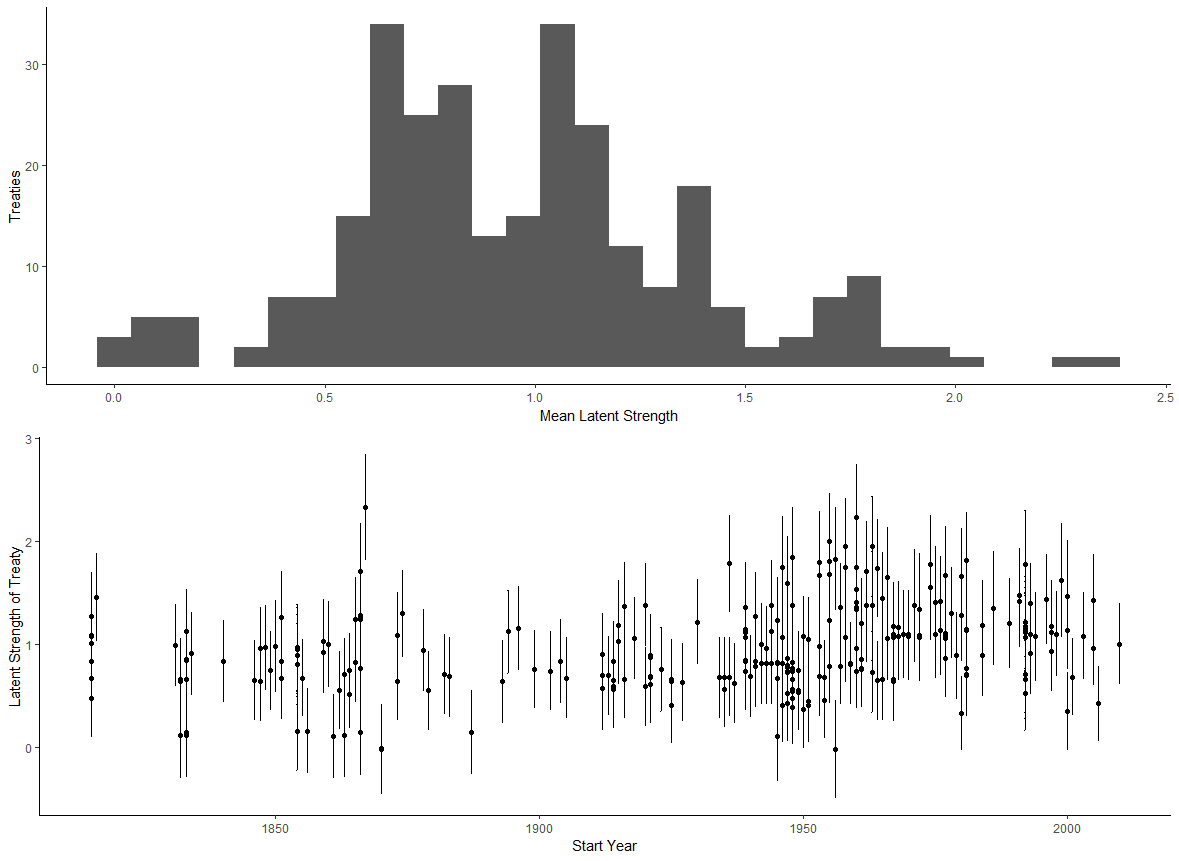
\includegraphics[width=0.95\textwidth]{../figures/ls-summary.png}
	\caption{Summary of latent measure of alliance treaty strength for 745 alliances from 1816 to 2016. The top panel is a histogram of the expected of alliance treaty strength. The bottom panel plots mean treaty strength (points) and the standard deviation (error bars) against the start year of the treaty.}
	\label{fig:ls-summary}
\end{figure}
	
	
The bottom panel of \autoref{fig:ls-summary} plots the posterior means and uncertainty in those estimates against the start year of the treaty. 
Even after accounting for posterior uncertainty, it is possible to distinguish between many strong and weak treaties. 
Institutionally weak treaties proliferated in the 20th century, with many non-aggression and consultation pacts. 


% Cases- especially strong and weak treaties
The values of the latent measure are not intrinsically informative. 
Differences in the latent measure between treaties on the scale are meaningful, however. 
The mean of treaty strength is 0.01, and the median is -0.10. 
This makes a 1938 consultation pact between France and Czechoslovakia (ATOPID 2120) typical. 


The weakest treaty is a neutrality and non-aggression treaty between Georgia and Kazakhstan (ATOPID 4476).  
An almost equally weak treaty between between Ukraine and India (ATOPID 4188) scores -1.36 on the latent measure.
The three strongest treaties are an 1867 alliance between Prussia and Hesse (ATOPID 1290), a 1955 treaty between Greece and Turkey governing relations in Cyprus and the United Arab Republic (ATOPID 3300).  
NATO scores 0.75, placing it in the upper edge of the third quartile of treaty strength.  


These examples show some face, concept, and discriminant validity of the latent measure. 
The UAR is a stronger commitment than non-aggression between India and Ukraine. 
The weakest treaties made few costly promises, while the strongest made substantial concessions. 
This measure distinguishes between weak and strong commitments. 
I now describe how and why I use a multilevel model to estimate the association between this measure of treaty strength and members military spending.  


\subsection{Multilevel Model} 


% Best fit for theoretical process. Can compare alliances. 
Multilevel modeling contains components of the specific and general research designs in previous research. 
Specific studies focus on responses to allied spending in particular treaties, while general studies in panel data rely on coarse aggregates of alliance participation.
In this model, I estimate the impact of each alliance treaty on member's military spending and the overall association between treaty strength and military expenditures. 
To overcome common estimation challenges, I fit this model using Bayesian estimation in STAN \citep{Carpenteretal2016}.\footnote{See the appendix for details of the weakly informative prior distributions and evidence of convergence.}


The multilevel model is more complex than traditional approaches. 
But added complexity has several benefits. 
Multilevel modeling connects the argument and research design. 
My predictions compare strong and weak treaties, so an alliance level regression in this multilevel model contains a corresponding coefficient.
Relying on a state-level proxy for alliance strength generates comparisons among states, which may produce misleading inferences. 


Multilevel modeling matches the structure of the data.
Alliances and states are separate levels of analysis. 
Connecting the alliance and state level of analysis allows us to infer how alliance variation impacts states' military expenditures. 


Added complexity facilitates detailed comparisons between alliances. 
The alliance-level regression gives a detailed picture of alliance characteristics that are correlated with alliance strength and military spending.
Partial pooling generates reasonable estimates of the impact of each alliance on members' military spending. 
Comparing patterns in these alliance-specific coefficients provides additional evidence to examine Hypotheses 1 and 2 as well as the importance of treaty strength. 


% Two separate but connected regressions
% State-level regression- alliances enter through spending matrix.
This multilevel model connects two distinct regressions. 
The base is a state-level regression, which is similar to a standard panel data regression.
A second alliance-level regression predicts parameters in the state-level regression, not unlike an interaction. 


The state-level regression starts with a distribution for the outcome:
\begin{equation}
y \sim student_t(\mu, \nu, \sigma)
\end{equation}
 
$y$ is growth in military spending. 
I model growth in spending with a t-distribution to address outliers.
$\sigma$ is analogous to the error term in a frequentist regression--- this captures unexplained variation in spending growth.  
$\mu$, the mean of the outcome, depends on several covariates.
\begin{equation}
\mu = \alpha + \alpha^{st} + \alpha^{yr} +\textbf{W} \gamma + \textbf{Z} \lambda
\end{equation}


Growth in spending is a function of an overall intercept $\alpha$, state and year varying intercepts $\alpha^{st}$ and $\alpha^{yr}$, and a matrix of state-level control variables \textbf{$W$}.
These components comprise a standard random effects model. 
The $\textbf{Z} \lambda$ term is the innovation, because it captures alliance participation.


\textbf{$Z$} is a matrix of state participation in alliances. 
Columns correspond to alliances, and rows to state-year observations. 
If a state is not part of an alliance, the corresponding cell of the matrix is zero.
If a state is part of an alliance in a given year, the corresponding cell is the log of total allied military spending. 


This is a quasi-spatial to capture alliance participation. 
I use total allied spending in the alliance participation matrix because more capable alliances provides more benefits.
Increasing allied capability makes promises of military support more valuable \citep{Johnsonetal2015}.  
Treaty design then modifies the value of allied capability.   
This measure also compares states inside and outside the treaty--- allied spending only applies to treaty members. 


Because the non-zero elements of $Z$ are allied spending, the $\lambda$ parameters capture alliance members' responsiveness to greater allied capability. 
Each alliance has a unique $\lambda$, which I give a common distribution. 
The second alliance-level regression predicts these $\lambda$ coefficients. 


% Alliance-level regression:
The second part of the multilevel model uses alliance characteristics to predict how allied spending is associated with growth in military spending. 
The $\lambda$ parameters are the dependent variable in a regression includes alliance treaty strength.
Therefore, I focus interpretation on this alliance-level regression, where: 

\begin{equation}
\lambda \sim N(\theta, \sigma_{all})
\end{equation} 
and 
\begin{equation}
\theta = \alpha_{all} + \beta_1 \mbox{Treaty Strength} + \textbf{X} \beta
\end{equation}

% Like an interaction between alliance and state-level factors 
Hypothesis 1 predicts $\beta_1$ will be negative among major powers, and Hypothesis 2 expects $\beta_1$ will be positive for non-major powers. 
In this alliance-level regression, $\textbf{X}$ is a matrix of alliance-level control variables and $\alpha_{all}$ is the constant.
Adding $\sigma_{all}$ ensures the predictions of $\lambda$ are not deterministic--- the alliance level regression contains an error term. 
Coefficients in the alliance-level regression are like marginal effects in an interaction. 
A change in treaty strength modifies $\lambda$, which alters growth in military spending. 


% Provide an example observation
Consider one observation as an example of how the model works. 
Growth in Argentina's military spending in 1955 depends on Argentina's economic growth, political regime, conflict participation, and rival military spending. 
Argentine participation in the Rio Pact and OAS also changes growth in spending. 


\begin{equation}
\begin{split}
& \mbox{Argentina 1955} = \mbox{Overall mean}
+ \mbox{Argentine Intercept} + \mbox{1955 Intercept} 
+ \mbox{Argentine Characteristics} \\
& + \lambda_{OAS} * \mbox{OAS Expenditure} + \lambda_{Rio} * \mbox{Rio Pact Expenditure}
\end{split} 
\end{equation}


$\lambda_{OAS}$ and $\lambda_{Rio}$ are modified by the alliance level regression. 
The institutional design and membership of these treaties alter the $\lambda$ parameter.
Alliances that Argentina does not participate in have no impact on growth in military spending. 


The multilevel model is highly interactive, which is appropriate for my conditional argument. 
Alliance characteristics modify the impact of allied spending on growth in state military spending. 
I now describe the sample and covariates in the multilevel model.  



\subsection{Sample and Covariates} 

% Sample of states and alliances: latter is restricted to treaties with military support 
I estimate this model on two sub-samples of states from 1816 to 2007. 
Alliance participation data comes from the ATOP project \citep{Leedsetal2002}. 
I focus on participation in defensive and offensive treaties, because prior studies of alliance participation also emphasize these treaties. 


% Because I think the DGP is different for large and small- split sample.
My argument suggests that major and non-major powers use alliances for different purposes.
Major powers focus on influence, non-major powers emphasize immediate territorial security.  
Therefore, the entire data-generating process connecting alliance participation and military spending should be different in major and non-major powers. 
To capture these differences, I estimate the model in separate samples- one sample of major powers, the other of non-major powers.
I employ the classification of major power status from the Correlates of War Project. 


The non-major power sample contains 8,668 observations. 
There are 930 major power observations. 
Though the major power sample is smaller and has fewer states, Bayesian estimation and partial pooling should give plausible estimates \citep{Stegmueller2013}. 


% Describe covariates at each level. 
In the state-level regression, I control for several correlates of alliance participation and military spending. 
State-level covariates include GDP growth \citep{Boltetal2018}, regime type, international war \citep{Reiteretal2016}, civil war participation \citep{SarkeesWayman2010}, annual MIDs \citep{Gibleretal2016}, rival military spending \citep{ThompsonDreyer2012} and a dummy for Cold War years.
I include growth in GDP instead of levels of GDP because GDP levels are non-stationary, and economic growth shapes the opportunity costs of military spending \citep{Kimball2010, Zielinskietal2017}.


Alliance level variables include my measure of treaty strength, number of members and share of democracies at time of formation \citep{Chibaetal2015}.
I also control for superpower membership--- whether the US or USSR participated in a treaty during the Cold War. 
Two dummy indicators of wartime alliances and asymmetric obligations \citep{Leedsetal2002} round out the alliance-level regression. 


Democratic membership in an alliance is associated both with limited obligations \citep{Chibaetal2015} and military spending \citep{DigiuseppePoast2016}, making it a particularly important alliance-level covariate.  
State and alliance-level controls for threat and conflict participation capture situations where states are more likely to seek allies. 
The next section describes the results.
 

\section{Results}


Results are based on 2,000 total samples from four chains, with 1,000 warm-up iterations. 
To facilitate model fitting, I employed a non-centered parameterization of the varying intercepts and a sparse matrix representation of \textbf{Z}. 
Standard convergence diagnostics indicate the chains adequately explored the posterior density.  


% note on interpreting Bayesian results
Because I use Bayesian modeling to estimate the association between treaty strength and growth in military spending, there are no conventional indicators of statistical significance. 
Instead, each coefficient has a posterior distribution--- the possible values of the coefficient conditional on the prior and observed data. 
Thus I calculate the positive and negative posterior probability for the treaty strength coefficient to assess Hypotheses 1 and 2.


% show latent strength coefficient in each subset of data
\begin{figure}[htbp]
	\centering
		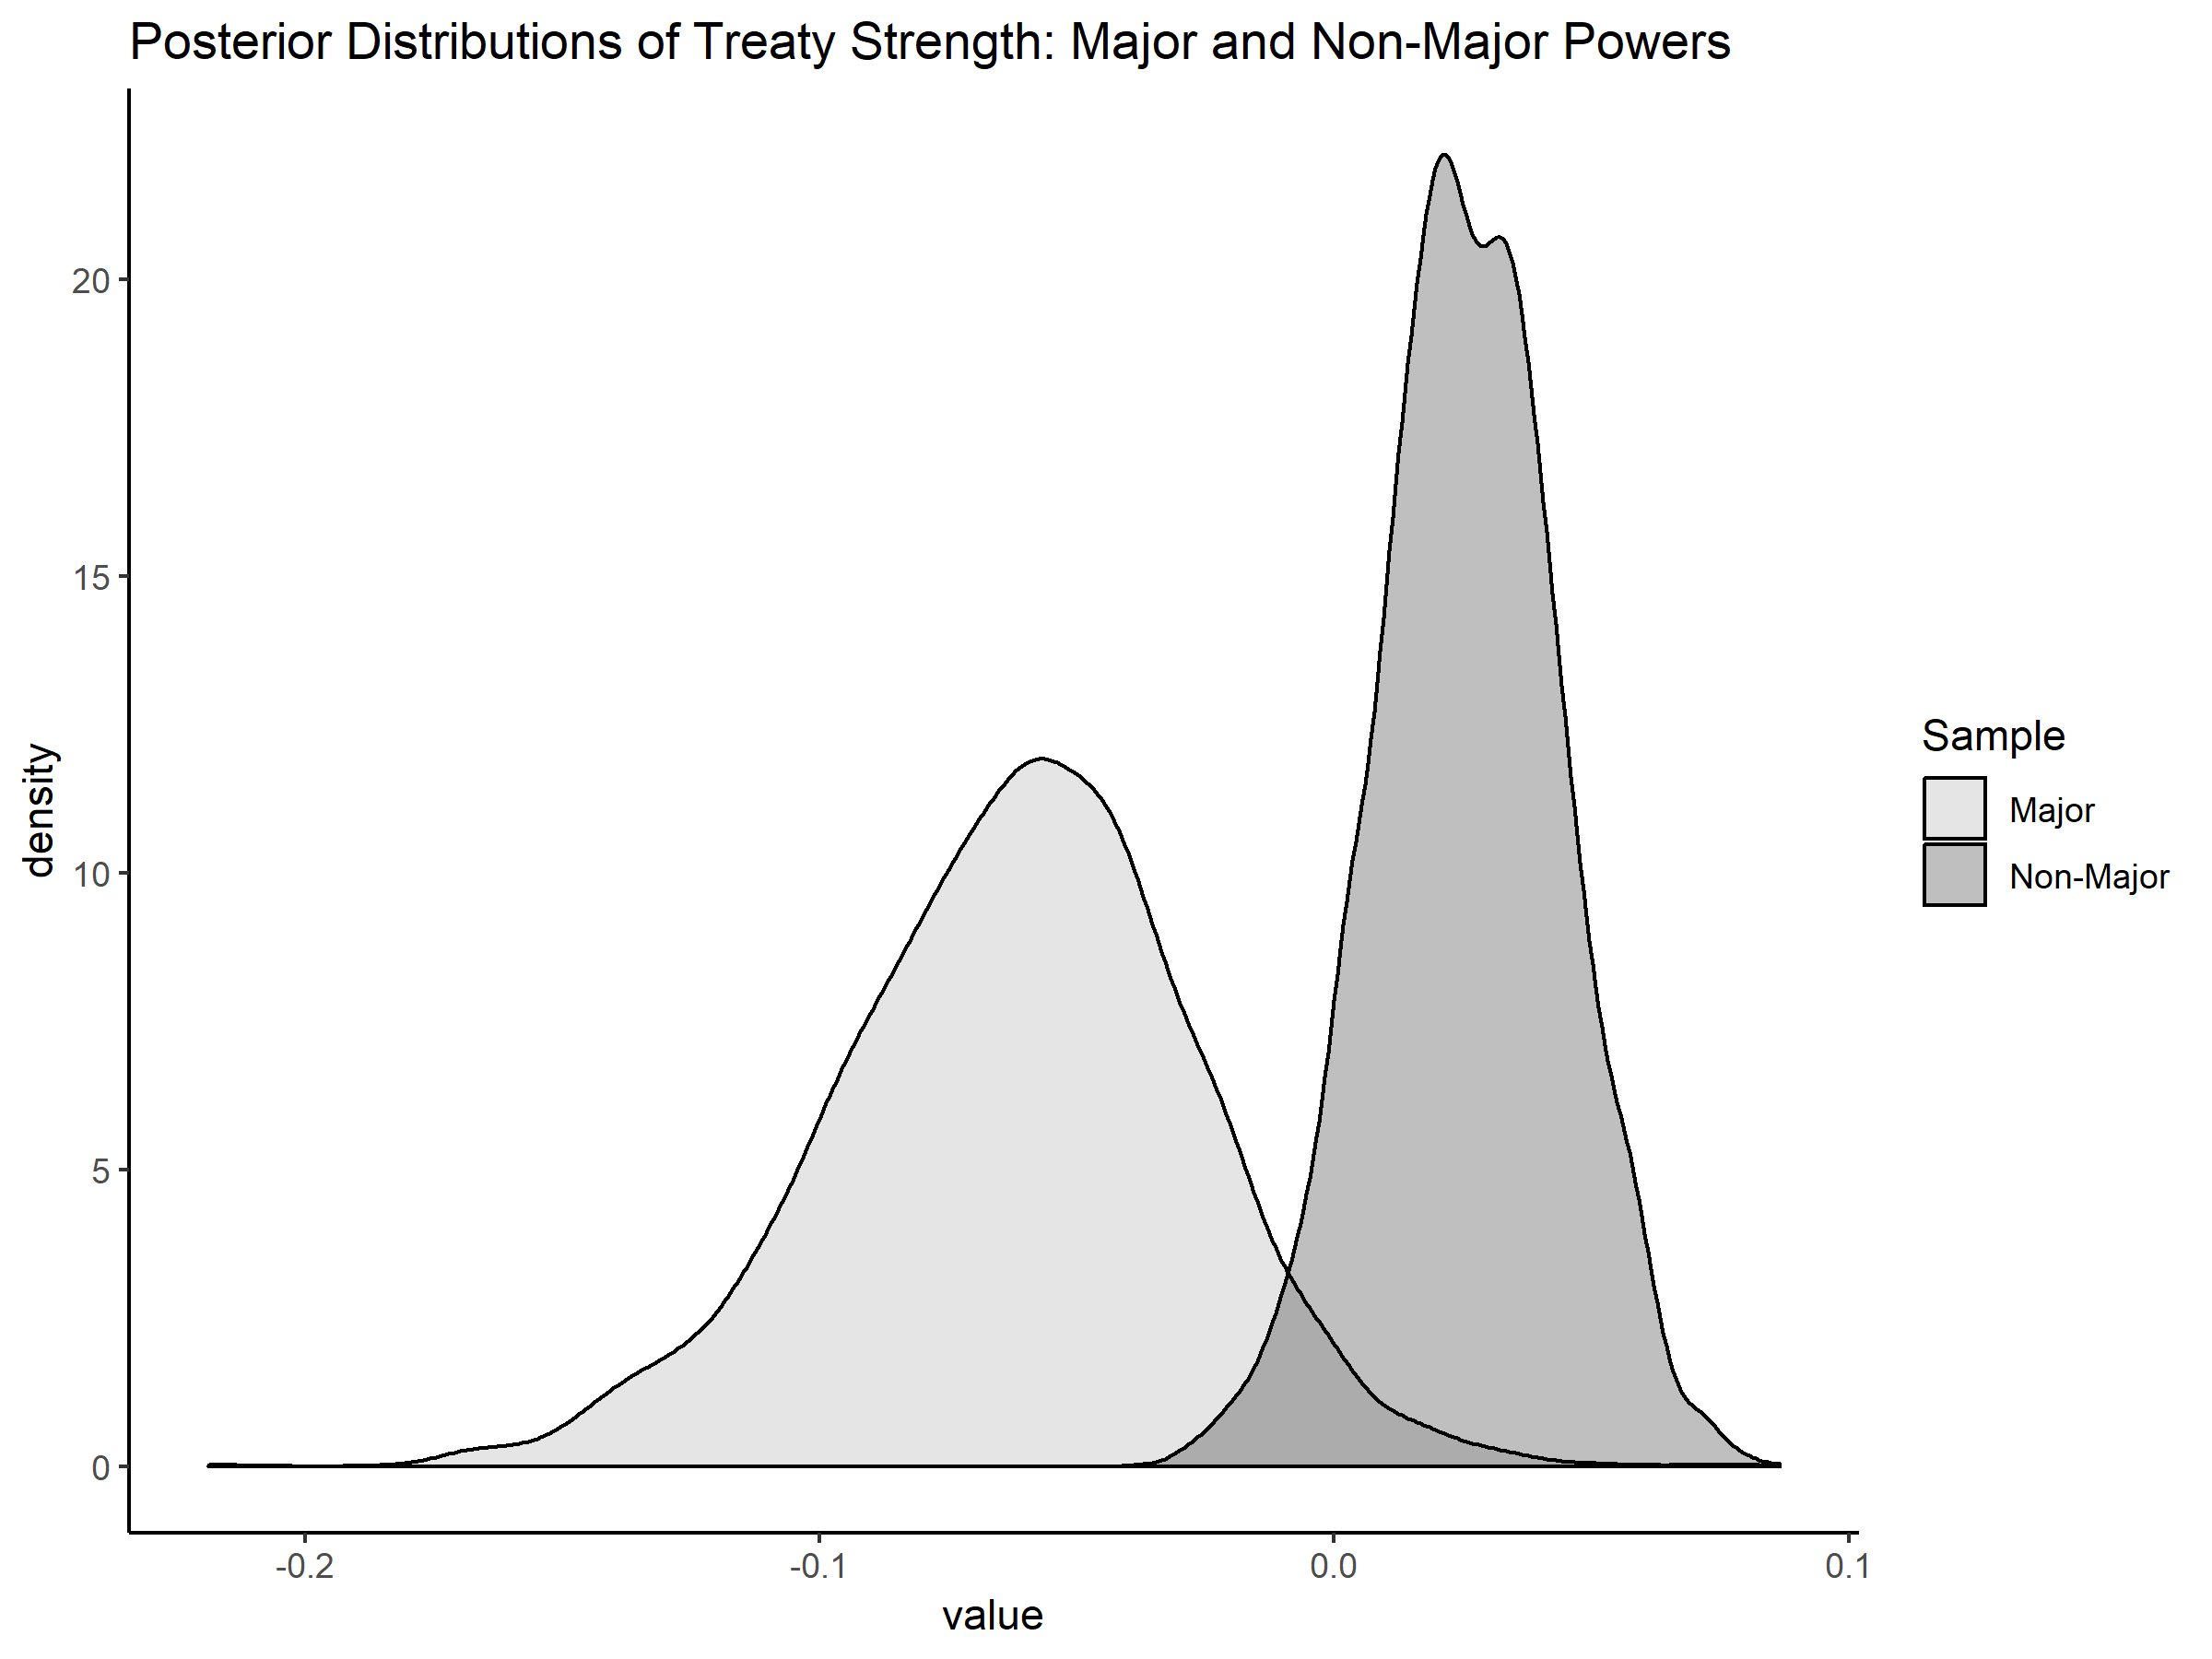
\includegraphics[width=0.95\textwidth]{../figures/str-dens.png}
	\caption{Posterior density of treaty strength coefficient in major and non-major power samples, 1816 to 2007. 96\% of the major power posterior mass is negative. 94\% of the non-major power posterior mass is positive.}
	\label{fig:str-dens}
\end{figure}


\autoref{fig:str-dens} plots the full posterior density of the treaty strength coefficients in the major and minor power samples.\footnote{The smaller sample for major powers produces more variance in all the coefficient estimates.} 
96\% of the posterior mass for major powers is negative. 
94\% of the posterior mass for minor powers is positive. 
There is little overlap between these two posteriors--- there is a 99\% chance that the association between treaty strength and military spending is larger for minor powers than major powers. 


These two coefficient estimates match the predictions of Hypotheses 1 and 2. 
For major powers, increasing treaty strength is associated with lower growth in military spending. 
Greater treaty strength is associated with higher growth in military spending for non-major powers.


How substantively important is treaty strength? 
Among major powers, the mean of the treaty strength coefficient is -0.05, and median growth in military expenditures is 0.04.\footnote{The median is a better summary of the dependent variable because large positive and negative outliers influence the mean.} 
So a one-unit increase in treaty strength offsets the typical annual growth in military spending. 


For non-major powers, the mean of the treaty strength coefficient is 0.03, and median growth in military expenditures is 0.06. 
Greater treaty strength increases growth in minor power military expenditures by about half of typical growth. 
Increasing treaty strength has a large substantive effect, relative to the scale of the data. 


We can also examine how much changing treaty strength influences on the overall association between changes in allied spending and growth in state defense spending. 
$\lambda_i$ measures the aggregate impact of changes in allied capability on military spending in for an individual treaty. 
If greater treaty strength has a large influence on the $\lambda$ parameters, there will be a clear trend in the value of $\lambda$ across the range of alliance treaty strength.
We should observe a negative trend in the expected value of $\lambda$ as treaty strength increases in major power alliances. 
Conversely, we should observe a positive trend in $\lambda$ for non-major power alliances. 


\begin{figure}[htbp]
	\centering
		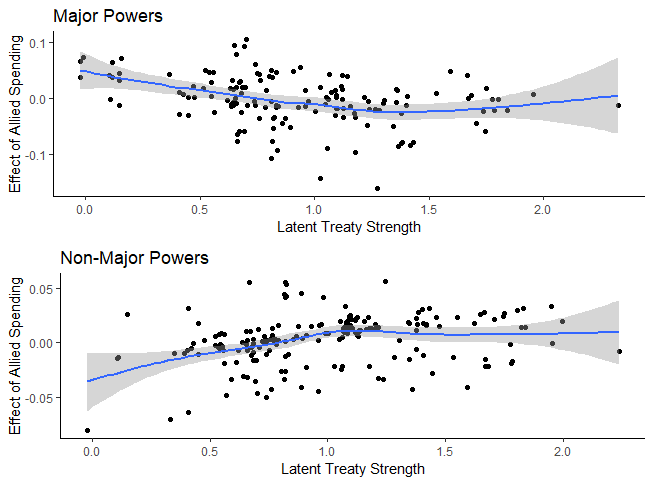
\includegraphics[width=0.95\textwidth]{../figures/lambda-ls-scatter.png}
	\caption{Scatter plots of trends in mean $\lambda$ parameters and treaty strength. $\lambda$ is the total impact of alliance participation on military spending. Trend lines estimated using linear regression. The top panel is major powers, where this is a negative trend between $\lambda$ and treaty strength. In the bottom panel the same trend is positive for non-major powers.}
	\label{fig:lambda-ls-scatter}
\end{figure}


\autoref{fig:lambda-ls-scatter} plots the expected value of $\lambda$ against treaty strength in the two samples. 
In the major power sample, there is a slight negative trend in the scatter plot.
For non-major powers, the trend is positive.
In both samples, the correlation between mean $\lambda$ and treaty strength is statistically significant. 


These trends match the predictions in \autoref{tab:arg-sum}.  
Weaker treaties tend to increase growth in defense spending for major powers, but that positive correlation falls as treaty strength increases. 
In non-major powers, the trend starts negative and becomes more positive as treaty strength rises. 


Because $\lambda$ captures the total impact of an alliance, this pattern suggests that increasing alliance strength has an important role. 
Even holding other alliance characteristics constant, alliance strength drives the overall effect of allied spending down for major powers, and up for non-major powers. 


\section{Discussion}


% Matches argument 
The above results match Hypotheses 1 and 2. 
Increasing treaty strength is positively associated with growth in military spending in non-major powers, who use the greater freedom of action in weak treaties to rely on their partners. 
Greater treaty strength is associated with lower growth in military spending for major powers, who use treaty strength and military capability as substitutes while seeking influence. 


% Precise interpretation: compares strong and weak alliances. Not treaty vs absence. 
These results contribute to the debate over whether alliance participation increases or decreases military spending. 
Dissension between the force multiplier and foreign entanglement views of alliances is based on competing claims about the purposes of alliances. 
These mutually exclusive assertions are inaccurate. 


My argument suggests claims that alliance participation only increases or decreases military spending are inappropriate. 
Instead, the association between alliance participation and growth in military spending depends on alliance member size and treaty strength. 
Alliance participation has heterogeneous effects because major powers and non-major powers employ treaties for different purposes. 
The conditional argument and research design show that alliance participation can increase or decrease spending for different states. 


Prior evidence is quite mixed, but comparing my results also requires renewed attention to specific and general research designs. 
Some of these studies compare states in a particular kind of alliances to those outside the treaty. 
Others examine responsiveness to allied military spending. 


How do my results compare to previous evidence on alliance participation and military spending? 
My key coefficient estimates compare strong and weak treaties, not states with a treaty to those without. 
However those estimates are like marginal effects- increasing treaty strength alters the effect of alliance participation.

 
$\lambda$ measures the impact of increasing allied spending \textit{for states in a treaty}. 
These parameters capture the impact of alliance participation only for treaty members. 
Therefore, a comparison between treaty members and non-members is included in the statistical model. 
Greater treaty strength decreases the association between alliance participation and growth in military expenditures for major powers, and increases it for non-major powers. 


% limitations of RD
There are several limitations to this paper.
The argument does not address the domestic political economy of military spending. 
My argument reduces domestic politics to the opportunity costs of military spending assumption. 


In the research design, measures of military spending are noisy and contain substantial measurement error. 
There is also a great deal of missing data in the 1816--2007 time frame of this study. 
I plan to check the robustness of my results to these issues in the near future by adding measurement error to the outcome and imputing missing data.


The multilevel model only incorporates time-invariant alliance characteristics, save for changing capabilities in the membership matrix. 
So I measure share of democratic members and the number of members at time of formation. 
Allowing time-varying alliance characteristics might improve the statistical model. 


% Strategic treaty design
Strategic alliance design is the last major weakness of the research design. 
Non-random selection into different kinds of alliances might lead to systematic differences between members that are not controlled for in my statistical model. 
I attempted to control for correlates of alliance treaty strength, especially democracy, but oversights remain possible. 



\section{Conclusion}


% Start conclusion 
This paper presented an argument and empirical evidence linking alliance participation and military expenditures. 
I explain when alliance participation is associated more or less growth in military spending, addressing a debate between competing views on this question. 
For major powers, greater treaty strength leads to lower growth in spending. 
Non-major power growth in spending is positively correlated with alliance treaty strength. 
I provide evidence for these predictions using a new measure of alliance treaty strength and a multilevel model. 


% Add paragraph on distributional consequences.
Changes in military spending growth have distributional consequences in the domestic economy. 
So the design of international alliances alters the domestic political economy of member states. 
Non-major powers must then face the opportunity costs of additional defense spending in strong treaties.
Major powers can use strong treaties to reduce to domestic costs of their foreign policy ambitions.  


% Next steps: extend argument to other treaty characteristics
There are several next steps for research on alliances and defense effort. 
One is extending the argument to other alliance characteristics. 
If major and non-major powers employ alliances for different ends, then other alliance characteristics may have different impacts on military spending. 
Large and small states might use wartime and asymmetric treaties differently, for instance. 


% Next steps: More interp of lambdas
Another task for future research is making more detailed comparisons of the $\lambda$ parameters. 
Each $\lambda$ captures the aggregate impact of alliance participation for a treaty.
As such, these parameters provide a novel measurement, and additional evidence of when alliance participation increases or decreases military spending. 


% Case studies
The multilevel model estimates do not establish causality. 
But the $\lambda$ parameters can guide case selection for a process-tracing analysis to corroborate the regression results.
One possible design is selecting the five largest and smallest $\lambda$ values for major and minor powers, and determining whether the connection between alliance participation and military expenditures matches the theoretical process.


% ML model and other cases of multiple membership 
The research design in this paper can address other research questions.
If scholars are interested in a class of international organizations and states are members in multiple organizations, the multilevel model addresses multiple membership.
Scholars can use this approach to estimate the unique impact of each organization and organizational characteristics on state-level outcomes. 
In international political economy, scholars might apply this model to trade agreements. 
Studies of international law could examine the impact of membership in different conventions and international organizations on human rights. 


% The argument indicates tradeoff
The argument and evidence suggests that major and non-major powers each face a tradeoff in alliance treaty design. 
Major powers tradeoff between the risk of entrapment and greater influence in strong treaties. 
Non-major powers sacrifice freedom of action for greater security as treaty strength rises. 


% Implications for policy. 
These twin tradeoffs have important consequences for policy debates.
The United States has a long history of decrying ``free-riding'' by allies who provide too little for their own defense \citep{Lanoszka2015}. 
But allies may be able to free-ride because the US prefers to form relatively weak alliance commitments. 
``Entangling alliances'' can provide greater influence to curb allied free-riding. 


Strong formal commitments can help restrain free-riding. 
Therefore, growing institutionalization of NATO, including the agreement for all allies to spend at least 2\% of GDP on defense, may be effective. 
However, treating alliances between major and non-major powers as a public good and low defense effort as free riding, is inaccurate. 
Asymmetric alliances produce different goods for different members. 
Major powers seek influence, while non-major powers secure their homeland. 


The US could use stronger formal commitments as a substitute for greater defense effort in reassuring allies.
The danger is that making stronger commitments might create a situation where obligations exceed capabilities \citep{Kennedy1987}. 
Emboldening junior partners with a strong treaty might have deterrent value \citep{Bensonetal2014}, or increase the risk of conflict \citep{Benson2012}. 

 
% tie it all together
The connection between alliance participation and military expenditures depends on state size and the strength of the treaty.  
Alliance participation does not exclusively increase or decrease military spending.  
Both the force multiplier and foreign entanglement views of alliance participation are correct in different circumstances. 




\singlespace
 
\bibliography{../../MasterBibliography} 





\end{document}
